\documentclass[a4paper]{article}
\usepackage[latin1]{inputenc}
\usepackage[english]{babel}
\usepackage{graphicx}
\usepackage[linewidth=1pt]{mdframed}
\usepackage{tikz-qtree}
\usepackage{algorithm}
\usepackage{algorithmic}
\usepackage{amsmath}


\usepackage[margin=2cm]{geometry}

\title{iMSG: Guiding language evolution by the need to express}
\author{Michael Cabot\\6047262 \and Sander Latour\\5743044}

\begin{document}
\maketitle
\section{Introduction}
\cite{zuidema2003poverty} \cite{batali1999negotiation}
In language learning, communication between a parent and a child typically starts with a semantic message (from now on refered to as the \emph{intention}) that the parent wants to share with the child. In order to communicate the intention, the parent needs to express it into a specific language formalism according to grammar rules known to the parent. The child then receives that expression in combination with the expressed intention. Although many communication happens between a parent and a child where there is not an explicit transfer of the intention, we focus on the part of language learning where the verbalized intention is somehow pointed out in other ways than verbal language (e.g. by ensuring a similar observation). Based on earlier communications together with the current one, the child attempts to induce structural grammar rules on how to parse and generate expressions.
\textbf{TODO: language evolution, iterative process between parent and child. progress made, especially by zuidema in reducing number of restrictions and assumptions. however problem in ever-decreasing grammar size}

The authors believe that the necessity to express a certain set of intentions will take care of the decreasing complexity of the grammar in a more natural way. The hypothesis is that by providing the parent with a list of intentions it needs to express, the iterated language evolution will optimize the language without reducing it to triviality. In order to test this hypothesis, this paper presents a semantic-driven iterated language learning framework based on both the work of \cite{zuidema2003poverty} on language evolution and the work of \cite{batali1999negotiation} on inducing semantic grammars from observations.

This paper is structured as follows. Section \ref{sec:system_overview} describes the system that was build. In section \ref{sec:experiments}, the experiments are described that were conducted to test the hypothesis. The results of these experiments are discussed in section \ref{sec:results}. Section \ref{sec:conclusion} concludes the results in this paper. And in section \ref{sec:discussion} the research is discussed.

\section{Related work}
%explain batali
%explain zuidema
%explain how this paper differs
\section{Notation and Vocabulary}
\begin{description}
    \item[formula] A formula $f$ consists of a predicate, denoted as $pred(f)$, and zero or more arguments, denoted as $args(f)$. The number of arguments is defined by the type of the formula, denoted by $type(f)$, which in this paper is either \verb|PropertyFormula| or \verb|RelationFormula| with one and two arguments respectively. For example, the formula \verb|(snake, 1)| has $pred($\verb|(snake,1)|$)$ = \verb|snake|, $args($\verb|(snake,1)|$)$ = $[1]$ and $type($\verb|(snake, 1)|$)$ = \verb|ProperyFormula|.
    \item[intention] An intention is a set of formulas that as a whole contains some semantic message. For example, an intention could contain \verb|[(tweety, 1), (see, 1, 2), (pussycat, 2)]| to express that tweety sees a pussycat. Intentions can be combined with other intentions by merging the sets.
    \item[rule] A rule $r$ is similar to an unnormalized PCFG rule. The left-hand-side of the rule, denoted by $lhs(r)$, is an intention. The right-hand-side of the rule, denoted as $rhs(r)$, is a set of intentions that together combine into $lhs(r)$. Linked to the rule is the cost of using the rule, denoted by $cost(r)$, which inversely relates to the probability of that rule being used.
    \item[argument mapping] For each intention $m$ in $rhs(r)$ there is an argument mapping that describes the transformation between the arguments of $m$'s formulas and the corresponding formulas in $lhs(r)$. For example, in figure \ref{fig:rule} the argument of [(tweety, 1)] remains the same while the arguments of [(see, 1, 2),  (pussycat, 2)] are inverted.
    \item[lexical rule] A lexical PCFG rule $r_l$ differs from normal rules in that the left-hand-side contains only one formula and $rhs(r_l)$ is a string of characters (i.e. a word). In this paper, $lhs(r_l)$ will for lexical rules denote the only formula in the left-hand-side. As a result, $type(lhs(r_l))$ will denote the type of the single formula in $lhs(r_l)$.
    \item[grammar] A grammar $G$ consists of all rules and lexical rules. The subgrammar $G_l$ is a subset of $G$ and contains only the lexical rules from $G$.
% argument mapping
\end{description}

\begin{figure}[h!]
\centering
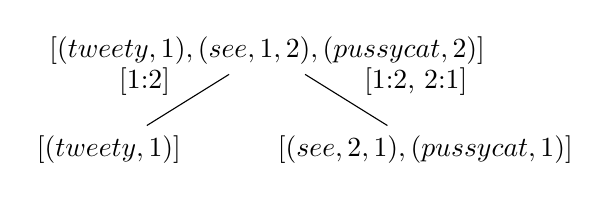
\begin{tikzpicture}[
   level distance=1.25cm,sibling distance=1cm,
   edge from parent path={(\tikzparentnode) -- (\tikzchildnode)}]
\Tree
[.\text{$[(tweety, 1), (see, 1, 2), (pussycat, 2)]$}
    \edge node[auto=right,pos=.6] {[1:2]};
    [.\text{$[(tweety, 1)]$}
        ]
    \edge node[auto=left,pos=.6] {[1:2, 2:1]};
    [.\text{$[(see, 2, 1), (pussycat, 1)]$} 
        ]
]
\end{tikzpicture}
\caption{A contex-free rule with argument mapping.}
\label{fig:rule}
\end{figure}

\section{System overview}
\label{sec:system_overview}
In order to explore the effect of this paper's approach and the validaty of the hypothesis, a computer simulation was designed and implemented. The computer simulation consisted of three main parts: \emph{generating intention}, \emph{expressing intention} and \emph{inducing grammar}. These parts will be described in the following sections.
% image depicting the general outline (parent -> child, iterated loop)
\subsection{Generating intention}
Three different methods were developed to obtain an intention to express. The first one is simply by taking a uniform random sample from a fixed set of intentions. The other two methos are \emph{predicate sampling} and \emph{template sampling}.
\subsubsection{Predicate sampling}
\label{sec:predicate_sampling}
A variation to having a predefined set of intentions is to only sample from predefined templates. These templates consist of placeholders that specify the type of formulas that can be ingested and the arguments that the formula wil have. For example, the template \verb|[(PropertyFormula, 1), (RelationFormula, 1, 2), (PropertyFormula, 2)]| allows for intentions that contain two properties and a relationship between them. A possible instantiation of this template is \verb|[(snake, 1), (bite, 1, 2), (pig, 2)]|. The templates ensure a certain complexity in the intention, without fully specifying it. The instantiation of the template is done by sampling formula predicates from the grammar that fit the specified type. The probability density function for this sampling is defined by the inverse cost of the lexical rule related to each formula. In order to deal with the situation where the grammar is still small and the amount of existing predicates in the grammar is limited or none, an exploration rate $\epsilon$ is introduced. The exploration rate defines the chance that a uniform sample is drawn from the set of unused (i.e. unknown to the parent) predicates instead of sampling them from the grammar. The instantiation of a template by sampling is described in the following algorithm:
\begin{mdframed}
    \textbf{Procedure 1} \textsc{PredicateSampling}\vspace{0.2cm}\hrule\vspace{0.2cm}
\noindent For each placeholder $t_i$ in template:
\begin{enumerate}
    \item Draw random number $\theta$, where $0 \leq \theta < 1$
    \item Initialize cumulative probability $p \gets 0$
    \item Initialize the set of unused formula predicates $U$ to the predefined set of all possible predicates of $type(t_i)$
    \item Define grammar subset $G_l'$ as $\left\{r \in G_l | type(lhs(r)) = type(t_i)\right\}$
    \item Calculate normalization constant $Z = \sum\limits_{r \in G_l'} \frac{1}{cost(r)}$
    \item For each lexical rule $r_l \in G_l'$:
        \begin{enumerate}
            \item Remove $pred(lhs(r_l))$ from $U$
            \item $p \gets p + \frac{1-\epsilon}{cost(r) \cdot Z}$, where $\epsilon$ is the exploration rate
            \item If $p \geq \theta$ then \textbf{insert} $pred(lhs(r_l))$ and \textbf{return}
        \end{enumerate}
    \item If $U \neq \emptyset$ then \textbf{insert} a random predicate from $U$ and \textbf{return}
    \item $\epsilon \gets 0$
    \item Go to step one
\end{enumerate}
\end{mdframed}
\subsubsection{Template sampling}
One set further than predicate sampling in fixed templates, is to also sample the templates from the grammar. The probability density function for templates is inversely related to the sum of the cost of all the rules that instantiate the template in their left-hand-side. Furthermore the probability of a template $t$ is normalized for the number rules needed to construct the instantiation using the normalization term $2 \cdot \left|\left|t\right|\right| - 1$, which is derived by combining the number of lexical rules ($\left|\left|t\right|\right|$) with the number of rules needed in the parse tree to reach the top ($\left|\left|t\right|\right|-1$). In order to deal with the situation where the grammar is still small and the amount of instantiated templates in the grammar is limited or none, the same exploration rate $\epsilon$ is used as in section \ref{sec:predicate_sampling}. Once a template is sampled, it can be instantiated using the earlier described \textsc{PredicateSampling} procedure. The sampling of a template is described in the following algorithm:
\begin{mdframed}
    \textbf{Procedure 2} \textsc{TemplateSampling}\vspace{0.2cm}\hrule\vspace{0.2cm}
\begin{enumerate}
    \item Draw random number $\theta$, where $0 \leq \theta < 1$
    \item Initialize cumulative probability $p \gets 0$
    \item Initialize the set of unused templates $U$ to the predefined set of all possible templates
    \item Calculate normalization constant $Z = \sum_{r \in G} \left[ \frac{1}{cost(r) \cdot 2 \cdot \left|\left|lhs(r)\right|\right| - 1} \right]$
    \item For each rule $r \in G$:
        \begin{enumerate}
            \item Convert the intention $lhs(r)$ to template $t$ by replacing the formula predicates with their type
            \item Remove $t$ from $U$
            \item $p \gets p + \frac{1 - \epsilon}{cost(r) \cdot 2 \cdot \left|\left|lhs(r)\right|\right| - 1}$, where $\epsilon$ is the exploration rate
            \item If $p \geq \theta$ then \textbf{return} $t$
        \end{enumerate}
    \item If $U \neq \emptyset$ then \textbf{return} a random template from $U$
    \item $\epsilon \gets 0$
    \item Go to step one
\end{enumerate}
\end{mdframed}
\subsection{Parent: Expressing intention}
Once an intention has been generated it needs to be expressed. Each formula predicate in the intention is converted into a string of characters. If the formula's predicate has a related lexical rule in the parent's grammar (i.e. is known to the parent), then the word stored in the right-hand-side of that lexical rule will be used to express that predicate. If the formula's predicate is not yet part of the parent's lexicon, then a string of random sampled characters will be generated instead. This string will be between the 4 and 8 characters long. The entire expression is a combination of the expressions for each formula in the intention.
% show example observations

\subsection{Child: Inducing grammar} % michael
The child receives an observation of the parent that contains an intention and a sentence that represents the intention. The child will try to interpret the sentence and derive multiple possible intentions. This is done by first substituting words with their corresponding intentions and then substituting these intentions using the rules in its grammar until a single intention remains that covers the whole sentence. A derivation consists of the list of rules that were used to cover the whole sentence. If a sentence is ambiguous, then multiple derivations with different intentions can be derived. The rules in the derivation whose final intention matches the intention of the observation are reinforced. The rules of the derivations that did not match the observation's intention but were cheaper to construct than the correct derivation are discouraged. When a rule is reinforced its cost is decreased according to equation \ref{eq:reinforce}:
\begin{equation}
cost(r) \leftarrow cost(r) - r*cost(r)
\label{eq:reinforce}
\end{equation}
where $r$ is the reinforcement parameter. The more a rule is used in a correct derivation the more its cost is reduced and the more likely it is used in another derivation. A rule is discouraged according to equation \ref{eq:discourage}:
\begin{equation}
cost(r) \leftarrow cost(r) + d
\label{eq:discourage}
\end{equation}
where $d$ is the discouragement rate.

The child's parser needs to cope with the fact that its grammar does not necessary contain the rules needed to parse a sentence. The authors extend the viterbi chart parser such that new rules can be created on the fly by either modifying existing rules in the grammar or by constructing entirely new rules. 

\subsubsection{ViterbiX} % michael
% TODO explain definition derivaiton.
The viterbi algorithm is a dynamic programming algorithm that finds the single most likely context-free derivation $T^*$ of a sentence $U$ given a Probabilistic Context Free Grammar (PCFG) $G$: $T^* = \arg \max_{T \in G(U)} P(T|G)$. The viterbi algorithm takes as input a sentence of length $n$ and a PCFG in Chomsky Normal form\footnote{TODO explain?} to create a parse forest: a chart that compactly represents the best derivations for each span in the sentence. A span ranges from word $i$ (inclusive) to word $j$ (exclusive), which will be denoted as $[i,j)$. A sentence is parsed bottom-up by substituting two adjacent non-terminals with spans $[i,k)$ $[k,j)$ with a single non-terminal with span [i,j), according to the rules in $G$. This process is repeated until a node with span $[0,n)$ is found, i.e. a node that covers the whole sentence. In order to retrieve the context-free rules used in a derivation, the $lhs(r)$ that is added to the chart at span $[i,j)$ also contains a pointer towards the two intentions of $rhs(r)$ and their spans $[i,k)$ and $[k,j)$.

In our model a context-free rule has on its left-hand-side an intention which is divided into sub-intentions on its right-hand-side such that $pred(lhs(r)) =  \bigcup_{m \in rhs(r)} pred(m)$, where $pred(m)$ gives the set of predicates for each formula in intention $m$. Since viterbi requires the grammar to be in Chomsky Normal form, the grammar contains only binary and unary rules (lexical rules).  Two intentions $B$ and $C$ with adjacent spans can be substituted if the grammar contains a rule $A \rightarrow B, C$. Since the child is learning a grammar and initially has an empty grammar, it must sometimes create the rules needed for parsing. A rule can be created in 2 different ways:
\begin{description}
\item[Substitution] An existing rule $r$ in the grammar can be adjusted such that its right-hand-side corresponds with the intentions $M = \langle B, C \rangle$ that need to be parsed:
  \begin{itemize}
  \item By substituting the argument mapping of $rhs(r)$. The cost of changing an argument mapping is $c_{arg}$
  \item By substituting intentions in $rhs(r)$. The cost of a substituted rule $r_{sub}$ is $cost(r_{sub}) = cost(r) + \sum_{m \in M} (cost(m) + c_{sub}) \delta[m \notin rhs(r) ]$, where $c_{sub}$ is the cost of substituting an intention and $\delta[m \notin rhs(r) ]$ is 1 if $m$ needs to be substituted, otherwise 0.
  \end{itemize}
\item[Creation] A new rule can be created by merging the intentions, such that $B\cup C \rightarrow B, C$ for any argument mapping. The cost a merged rule $r_{merge}$ is $cost(r_{merge}) = cost(B) + cost(C) + c_{merge}$, where $c_{merge}$ is the cost of merging. A lexical rule can be created by placing a word in the right-hand-side of the rule and its intention on the left-hand-side. It is assumed that the index of each formula in the intention of the given observation corresponds with the index of each word of the sentence. The cost of a new lexical rule is $cost(r_l) = c_l$.
\end{description}

Viterbix is an extension of viterbi that uses \textit{substitution} and \textit{creation} of new rules to create an expanded grammar $G'$ that is able to substitute two adjacent intentions. Algorithm \ref{alg:viterbix} gives a general overview of the viterbix algorithm. On line 1 the chart is initialized with all lexical rules for each word in the given sentence. Then for each pair of intentions $\langle B, C \rangle$ in adjacent spans $[i,k)$-$[k,j)$ an expanded grammar is created. 
% TODO continue
Line 6 checks whether the cost of $A$ is lower than an equivalent intention present in the chart at $[i,j)$. If chart(i,j) does not contain $A$, then $cost(\cdot)$ returns infinite ensuring $A$ will be added to the chart.

\begin{algorithm}
\caption{ViterbiX general algorithm}
\begin{algorithmic}[1]
\REQUIRE sentence, $G$
\STATE chart $\leftarrow$ initialize(sentence, $G_l$)
\FOR{ $0 \le i < k < j \le n$ }
    \FOR{ $B \in chart(i,k)$ \AND $C \in chart(k,j)$ }
        \STATE $G' \leftarrow G.expand(B, C)$
        \FOR{ $A \in G'$ }
            \IF{cost(A) $<$ cost(chart(i,j).get(A)) }
                \STATE add A$\rightarrow$(B,k,C) to chart(i,j)
            \ENDIF
        \ENDFOR
    \ENDFOR
\ENDFOR
\RETURN chart
\end{algorithmic}
\label{alg:viterbix}
\end{algorithm}
\section{Experiments}
\label{sec:experiments}
\section{Results}
\label{sec:results}
\section{Conclusion}
\label{sec:conclusion}
\section{Discussion}
\label{sec:discussion}

\bibliographystyle{plainnat}
\bibliography{references}

\end{document}
